\chapter{Theoretical Backgrounds}
\textit{//TODO: Revise and move this chapter to appendix}

\nocite{DBLP:journals/corr/Lipton15}

This chapter presents the theoretical backgrounds in deep learning that act as foundation for all the models used in the thesis.
The first section introduces the concept of artifical neuron (or \textit{neuron}) - building block of modern artifical neural networks - and its learning procedures and algorithms including \textit{stochastic gradient descent} and \textit{backpropagation}. The second section describes the architecture of Convolutional Neural Network (CNN) - the infamous type of network that has achieved astounishing performance on numerous computer vision tasks such as classification, detection, segmentation, etc. Another type of neural network - Recurrent Neural Network (RNN), which is powerful for many tasks in natural language processing domain - is presented in the third section. 
\section{Artificial Neuron}

\begin{wrapfigure}{r}{0.35\linewidth}
	\vspace{-20pt} % reduce top space of the figure
	\label{fig:neuron}
	\centering
	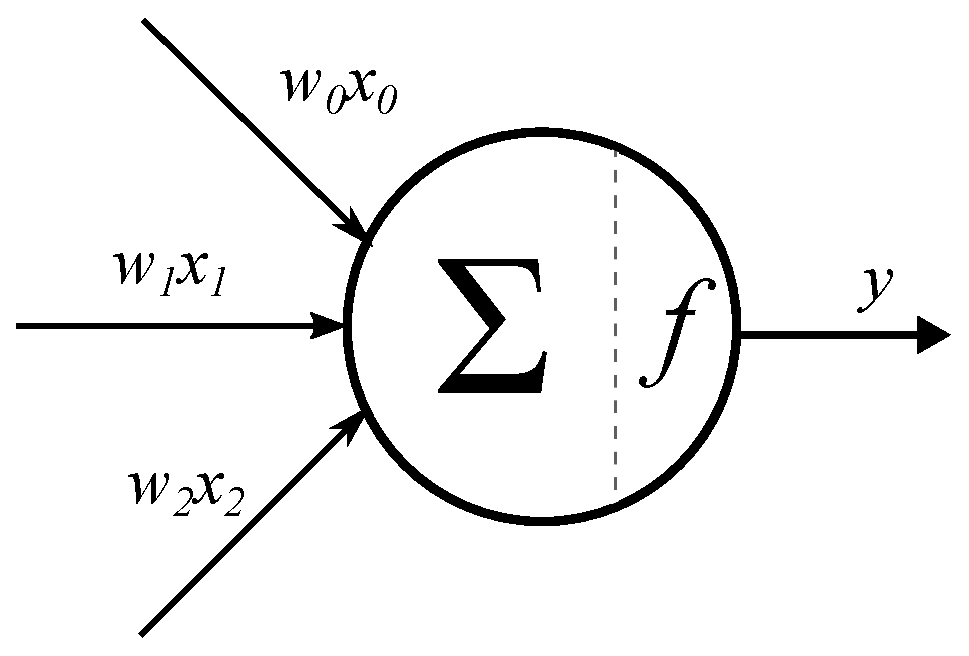
\includegraphics[scale=0.35]{Chapters/Fig/neuron.eps}
	\caption{A single artificial neuron}
	\vspace{-25pt} % decrease bottom space of the figure
\end{wrapfigure}

\subsection{Notations and Terminologies}

A neuron is a decisive device which takes several inputs and produces one ouput. Figure \ref{fig:neuron} depicts a neuron which takes three inputs and produces one ouput, where:
\begin{itemize}[noitemsep]
	\item $x_i$: the input to neuron
	\item $w_i$: the weight of input $x_i$
	\item $b$: the bias of neuron
	\item $\sum\left(w_ix_i + b\right)$: the activation of the neuron
	\item $y$: the output of the neuron
\end{itemize}

Here, the learnable parameters are weights $w_i$ and bias $b$. By varying those parameters, we can get different models of decision-making.

There are several types of activation functions often used in deep neural networks. They are listed in Figure \ref{fig:activation-function}
\begin{figure}[h]
	\centering
	\subfigure[Sigmoid function]{%
		$\begin{aligned}
			f\left(z\right) = \frac{1}{1 + e^{-z}}
			\end{aligned}
		$
	}
	\qquad
	\subfigure[Hyperbolic tangent function]{%
		$ \begin{aligned}
			f\left(z\right) = \tanh\left(z\right)
		   \end{aligned}
		$
	}
	\qquad
	\subfigure[Rectified linear function]{%
		$ \begin{aligned}
			f\left(z\right) = max\left(0,z\right)
		   \end{aligned}
		$
		% 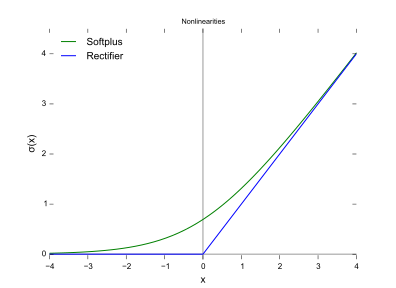
\includegraphics[width=\linewidth]{Fig/relu.svg}
	}
	\caption{Typical activation functions}
	\label{fig:activation-function}
\end{figure}

\subsection{Learning with a single neuron}
In general Machine Learning, the learning is the process to find out a hypothesis function $h\left(x\right)$ that best fits the test data set. It is often that the form of such function is chosen beforehand (e.g., linear, quadratic, etc.). 

\textit{//TODO: rewrite}
\section{Feed-forward Neural Network}
\begin{figure}
	\centering
	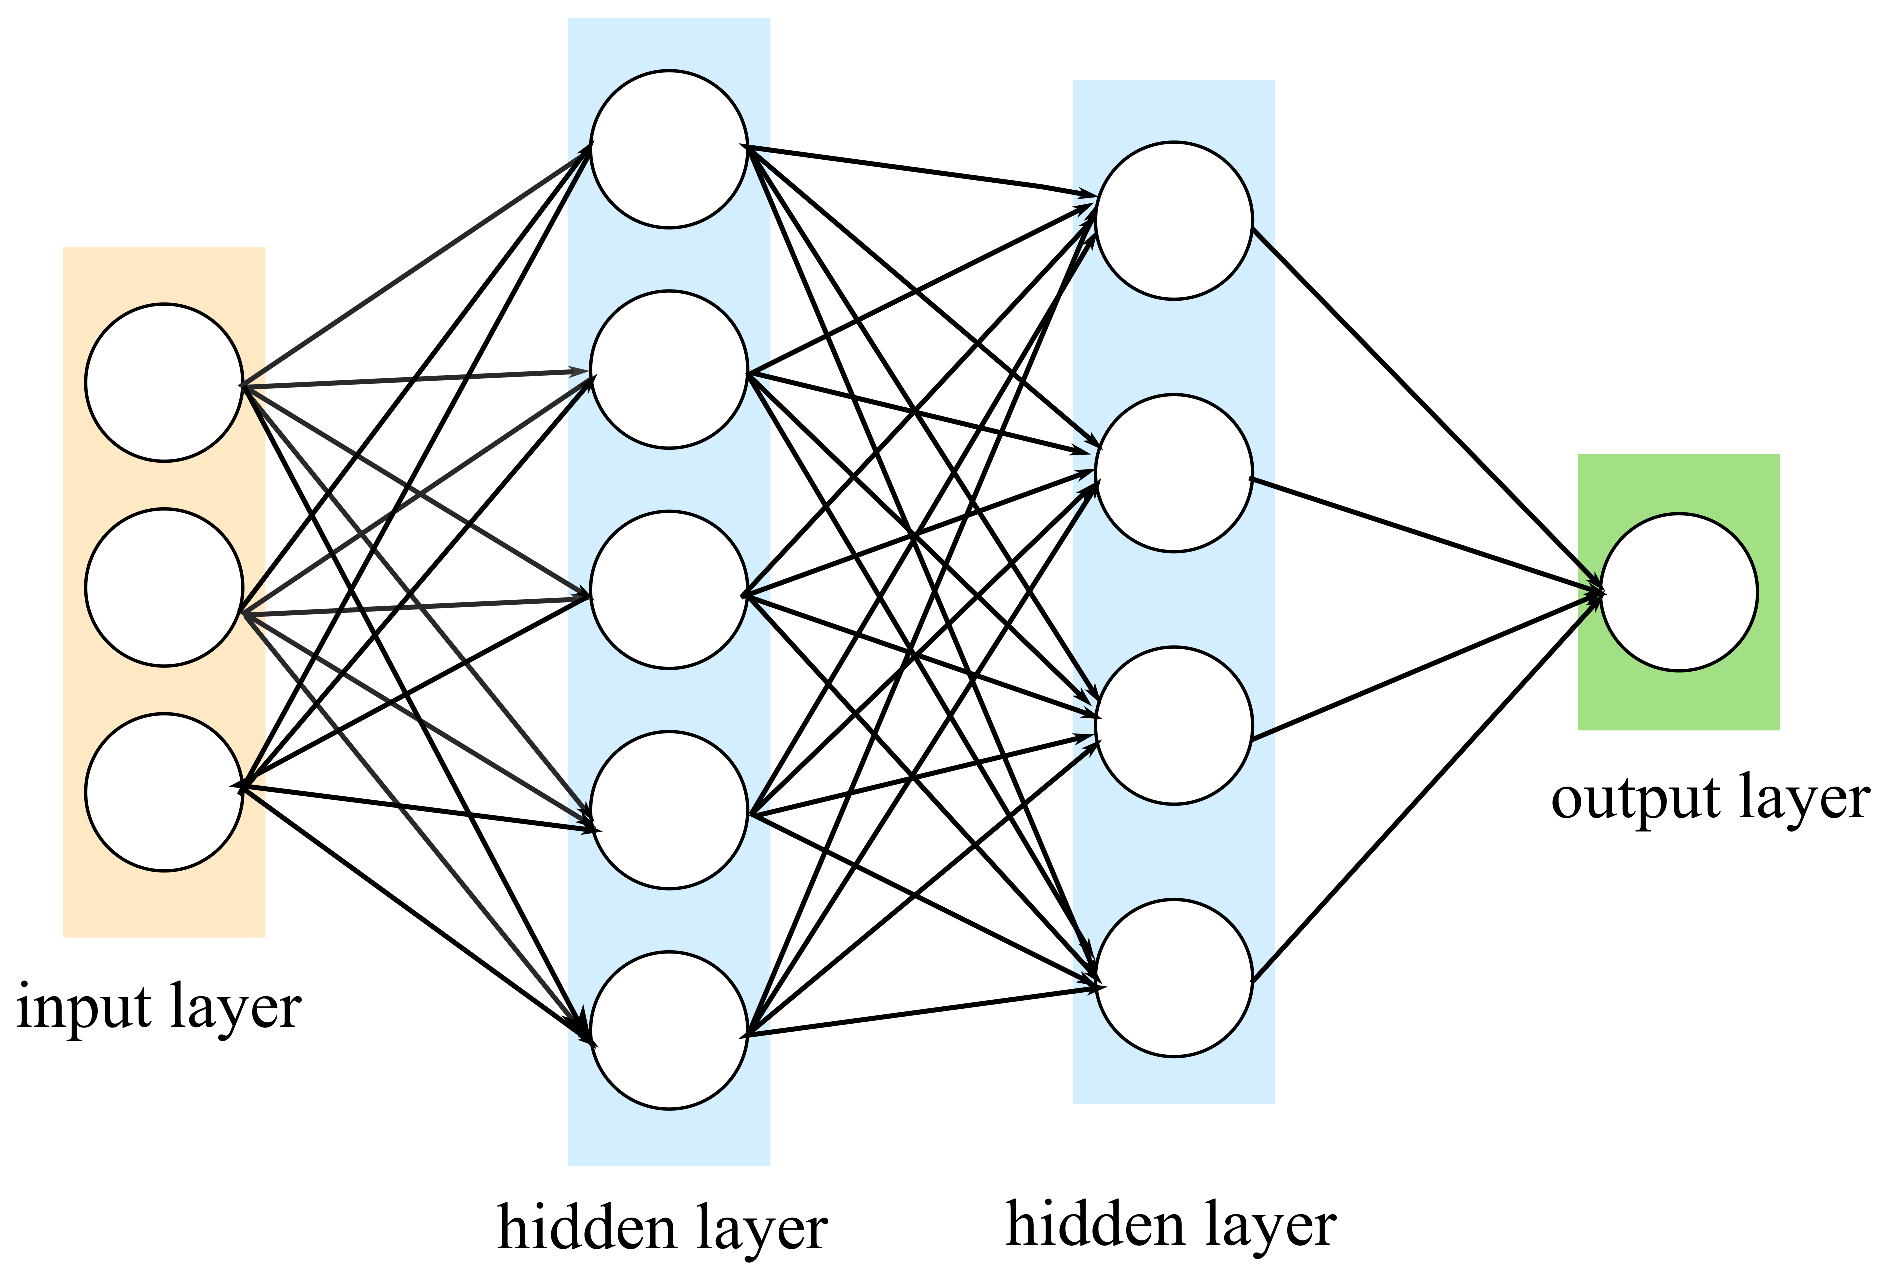
\includegraphics[width=0.75\linewidth]{Chapters/Fig/feedforward.eps}
	\caption{A feed-forward neural network consisted of four layers: 1 input layer, 2 hidden layers and one output layer}
	\label{fig:ff-net}
\end{figure}
Feed-forward neural networks (or \textit{Fully-connected neural networks}) are comprised of layers of neurons. Every neuron in $l$\textit{th} layer is connected to every neuron in $\left(l+1\right)$\textit{th} layer, but there are no connections between neurons within same layer nor connections between neurons in layer $\left(l+1\right)$ to neurons in layer $l$. Figure \ref{fig:ff-net} illustrates the architecture of a simple feed-forward neural network. There is a real-valued weight. Neuron $k$ in layer $l$ receives as input:

\begin{align*}
	x^l_k = b^l_k + \sum^{N_{t-1}}_{i=1} w^{l-1}_{ik}y^{l-1}_i
\end{align*}
The neuron then computes its output
\begin{align*}
y^l_k = f\left(x^l_k\right)
\end{align*}
where $f$ is any differentiable function of the neuron's total input. The neurons in the data layer just out the data.

Finally, we come up with a function 
\begin{align*}
	E\left(y^L_1, \dots, y^L_{N_L}\right)
\end{align*}
of the output that we would like the neural net to maximize (this can be seen as just another layer on top of the output layer), where $L$ is the number of layers in the neural network. $E$ should be differentiable so $\displaystyle\frac{\partial E}{ \partial y^L_k}$ is readily computable. Training the network consits of clampng the data neurons at the data and updating the parameters (the weights and biases) in the direction of the gradient. The derivatives can be computed as follows:
\begin{align*}
\frac{\partial E}{\partial w_{ik}^{l-1}} &= \frac{\partial E}{\partial x^l_k}y^{l-1}_i\\
\frac{\partial E}{\partial b^l_k} &= \frac{\partial E}{\partial x^l_k} 
\end{align*}
where
\begin{align*}
\frac{\partial E}{\partial x^l_k} &= \frac{\partial E}{\partial y^l_k} \frac{\partial y^l_k}{\partial x^l_k}\\
% \frac{\partial E}{\partial y^l_k} &= \begin{cases} 
% 										&\frac{\partial E}{\partial y^L_k} & \text{if} l = L \\
% 										&\sum^{N_{t+1}}{i=1} \frac{\partial E}{\partial x_i^{l+1}} w^l_{k_i} & \text{otherwise}
% 									 \end{cases}
\end{align*}
and $\displaystyle\frac{\partial E}{\partial y^L_k}$ is assumed to be readily computable. From this, derivatives with respect to all the weights and biases can be computed, working down from the top layer. This is know as the backpropagation algorithm. Typically, the gradient is averaged over a whole batch of images, and the the parameters are updated with this \textit{average gradient}. This is know as batch learning.

\section{Convolutional Neural Network}
\subsection{Overview}

\subsection{Convolutional layer}

\subsection{Nonlinear layer}

\subsection{Pooling layer}

\section{Recurrent Neural Network}